\chapter{Intuition Behind the Integral}
The point of the integral is to find the area under a curve. 
One of the interesting applications of integration is finding the displacement of an object - the displacement corresponds to an object's trajectory; that is, the area under a graph of velocity versus time is displacement.

While we don't actually need to do the following, this is generally what is happening. 

\begin{centering}
\begin{figure}[H]
\caption{Riemann Sum}
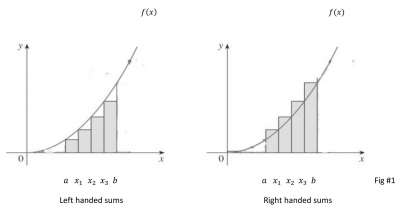
\includegraphics[scale=0.8]{../rieman.jpg}
\end{figure}
\end{centering}

Basically, we pick a specified width, let's say $w$. 
Then, we create several rectangles, with a width $w$ and a height that is just under the curve we are trying to find the area of. 
Then, we do this again, but this time the height is just above the curve. 
We take the average of the two numbers, and get the area of the curve. 
The smaller we make $w$, the more accurate the number, and at width $0$, we basically have lines, which fit the curve perfectly. 
This is the point of an integral.
\chapter{Basic Integration Rules}
Below is a table of some of the basic outputs of integrals. Some of these will make more sense after going through derivatives.

\begin{tabular}{l|l}
    $f(x)$ & $\int f(x) \, dx$\\
    \hline
     $0$ & $0+c$ \\
     $1$ & $x+c$ \\
     $D$ & $Dx+c$ \\
     $2x$ & $x^2 + c$ \\
     $x$ & $x^2/2 + c$ \\
     $x^2$ & $x^3/3 + c$ \\
     $x^n$ & $x^{n+1}/n+1 + c$
\end{tabular}

In these, $c$ and $D$ are constants and $x$ is some variable.

Note that after every integral, we must put $dx$ or $dt$ or $d$ and then whatever variable we are using in our integral. 
The second important thing to note is that these results have $c$ after them because they are ``indefinite'' integrals - that is, because we don't have a specific bound on the integral, we must add a constant $c$ to show that there is some range in what the answers will be. 
This is again something that will make more sense after going over derivatives.

So there are indefinite integrals, but there are also "definite" integrals. 
We write them as $\int^b_a$. Basically, let's say we have the integral $\int x \, dx$. 
We integrate the inside according to the table, getting $x^2/2$, but instead of adding the constant $c$, we then plug in $b$ and $a$ in for $x$ as follows: 
\begin{equation*}
    (b^2/2) - (a^2/2)
\end{equation*}

This gives our answer, and we do not need to put in $c$.

There is another important thing about integrals. For an integral such as $\int x+x \, dx$, we can change this into

\begin{equation*}
    \int x \, dx + \int x \, dx
\end{equation*}

We can also factor out constants; for example, given $\int 2x + 3x \, dx$, we can change this into 

\begin{equation*}
    2\cdot \int x \, dx + 3 \cdot \int x \, dx
\end{equation*}

Also remember that you can simplify within a problem; i.e., given $x(x^2 + x^3)$ you can then multiply and get $x^3 + x^4$. 
Finally, there is a helpful rule for integrals - the product rule. 
If you have a function $v(x)$ and a function $u(x)$, and you wish to find the derivative of $u(x)\cdot v(x)$, you can follow the rule $u\cdot v - \int v\frac{du}{dx}\, dx$.
\chapter{Derivatives and Integrals}
Derivatives and integrals are inverses of each other. 
That is, they undo each other, like division undoes multiplication and subtraction undoes addition. 
(This is called the "fundamental theorem of calculus".)
So, because when going from an integral back to a derivative there is some uncertainty which graph you are looking at (parallel lines, for instance, have the same slope, but they have different "heights"), you have to add the $c$ when solving an indefinite integral. 
\chapter{Formal Definition of an Integral}
\section{Summations}
A summation is a simple method of notation that shortens long repetitive addition operations. Let's look at an example:

\begin{equation}
\sum\limits_{n=0}^{n=5} 2n
\end{equation}

Here, the expression $n=0$ under the summation symbol means that to start the sum, we plug in $0$ for $n$. The expression $n=5$ on top means we continue until we have plugged in $5$ for $n$. Expanded, this summation means

\begin{equation}
2\times 0+2\times 1+2\times 2+2\times 3+2\times 4+2\times 5
\end{equation}

which means the answer is $30$. Think back to the section on the intuition behind integrals for why we need this. We're really summing up a bunch of small rectangles. 
\section{Formal definition of indefinite integrals}
\section{Formal definition of definite integrals}